\chapter{INTRODUÇÃO} \label{cha:introd}

Esta é uma série para apresentar o uso do template e não uma documentação da customização. Este documento pressume que você conheça algumas características de uso do LaTeX, caso não tenha nenhuma informação/formação, basta acessar o documento de documentação em pdf deste repositório. Nele você encontrará um curso básico de LaTeX para utilizar a customização sem muitas dificuldades.

Claro, a curva de aprendizado inicial é difícil de ser percorrida. Depois de se acostumar, fica mais simples e satisfatório.
\section{UTILIZAÇÃO DESTE TEMPLATE} \label{sec:util}

Veja que é necessário colocar os títulos do capítulo e da seção em caixa alta. É recomendado ter um texto entre as seções do documento.

Você pode digitar o texto e utilizar os recursos do LaTeX para colocar os elementos gráficos, tabelas, quadros, expressões matemáticas, siglas, símbolos, citações e referências. Foram configurados alguns comandos para facilitar o seu trabalho.
\subsection[Imagens]{Imagens e figuras}\label{ssec:imafig}

Para inserir uma figura com o comando \verb+\includegraphics+ para ficar de acordo com a normalização ABNT-UFPR:
\subsubsection{imagem}\label{sssec:imagem}

\verb+\imagem{Título da imagem}{largura}+ 

\verb+   {figura com sua localização }{Fonteda figura}+

\verb+   {label}{alguma nota}{alguma legenda}+

\begin{lstlisting}
\figura
{FIGURA DE TIPOS PARA IMPRESSAO}  % Titulo
{.75}                             % % da largura da linha
{fig/tipog.png}                   % caminho da figura
{\citefig{tipo2012}.}             % Fonte
{tipoex}                          % label = fig:tipoex
{Esta eh uma nota musical, 
 Esta eh uma nota musical e 
 Esta eh uma outra nota}          % Texto da Nota
{Nao quero colocar legenda.}      % Texto da Legenda
\end{lstlisting}

Para fazer referencia a esta figura, basta digitar \verb+\autoref{fig:tipoex}+.

Para inserir um elemento gráfico gerado/compativel com o LaTeX, você tem o comando imagem com 7 parâmetros:

\begin{lstlisting}
% simplificacao para colocar figuras
% ----------------------------------------------------------
%   Parametros
%    1 caption
%    2 percent textwidth
%    3 arquivo da figura
%    4 fonte
%    5 fig:label
%    6 nota
%    7 legenda

\figura
{FIGURA DE TIPOS PARA IMPRESSAO}  % Titulo
{.750}                            % %da largura da linha
{fig/tipog.png}                   % caminho da figura
{\citefig{tipo2012}.}             % Fonte
{tipoex}                          % label = fig:tipoex
{Esta eh uma nota musical. 
 Esta eh uma nota musical.
 Esta eh uma nota musical. 
 Esta eh uma nota e esta 
	eh uma outra nota}            % Texto da Nota
{Nao quero colocar legenda.}      % Texto da Legenda
\end{lstlisting}

Para fazer referência a esta figura, basta digitar \verb+\autoref{fig:tipoex}+

\begin{lstlisting}
% simplificacao para colocar imagens
% ----------------------------------------------------------
%   Parametros
%    1 caption
%    2 imagem tikz ou pgfplots ou outro elemento qualquer
%    3 fonte
%    4 fig:label
%    5 nota
%    6 legenda
\end{lstlisting}

\verb+\imagem{Titulo}{arg2}{fonte}{label}{nota(s)}{legenda(s)}+

\begin{lstlisting}
\imagem{Titulo}
	{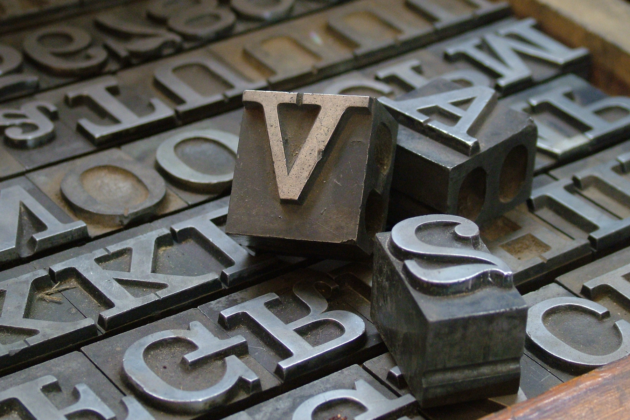
\includegraphics[width = 80mm]{fig/tipog}}
	{fonte}
	{label}
	{nota(s)}
	{legenda(s)}
\end{lstlisting}


\imagem{Titulo}{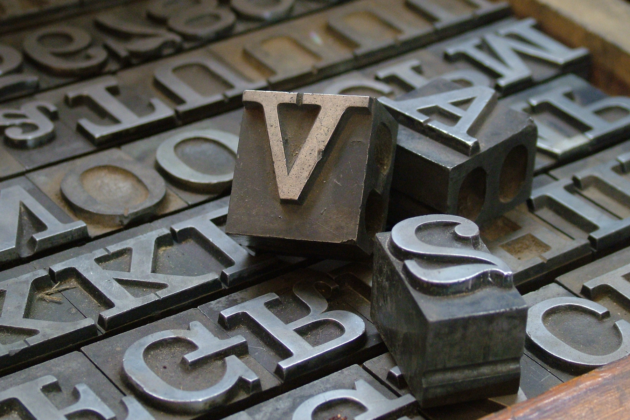
\includegraphics[width = 80mm]{fig/tipog}}{fonte}{label}{nota(s)}{legenda(s)}

Para fazer referência a esta figura é da mesma forma,\verb+\autoref{fig:label}+, \autoref{fig:label}

\subsection[Quadros e tabelas]{Quadros e tabelas}

Lembrando que quadros tem informações e são fechados lateralmente e verticalmente, tem a posição do título, fonte, nota e legenda diferentes da tabela.
\subsection[Quadros]{Inserir quadros}\label{ssec:quadros}

Para inserir um quadro são necessários 6 parâmetros:

\begin{lstlisting}
% ----------------------------------------------------------
%   Parametros
%    1 caption
%    2 elementos tabulados
%    3 fonte
%    4 qua:label
%    5 nota
%    6 legenda
\end{lstlisting}

Os elemento tabulados foram inseridos no ambiente tabular, com as laterais e parte superior e inferior fechados.

Este ambiente não quebra sua estrutura em páginas.

\begin{lstlisting}
\qquadro{Prefixos convencionados para referencias}
{\footnotesize
 \begin{tabular}{|l*{6}{|c}|}\hline
  \textbf{Elementos}:& 
       capitulos & secoes & 
       subsecoes & subsubsecoes &
       figuras   & imagens \\\hline
  \textbf{prefixos}:&
     cap &sec &
     ssec &sssec &
     fig & img\\\hline\hline
  \textbf{Elementos}:& tabelas &
     quadros & equacoes & exemplos &
     exercicios & questoes\\\hline	
  \textbf{prefixos}:&
     tab &    qua & 
     eq  &    exm & 
     exc &     que\\\hline\hline
  \textbf{Elementos}:& itens enumerados &
                       alineas&teoremas &
                       axiomas          & 
                       listagem         &\\\hline
  \textbf{prefixos}:&  inum & ali & teo & axi & lst &\\\hline
\end{tabular}}
{O autor(2021)}{quadrinho}{}{}
\end{lstlisting}

\qquadro{Prefixos convencionados para referencias}
{\footnotesize
 \begin{tabular}{|l*{6}{|c}|}\hline
  \textbf{Elementos}:& capítulos& 	seções&	subseções&	subsubseções&	
  figuras&	imagens \\\hline
  \textbf{prefixos}:&cap&sec&ssec&sssec&fig & img\\\hline\hline
  \textbf{Elementos}:&tabelas&	quadros&	
  equações& exemplos& exercícios & questões\\\hline	
  \textbf{prefixos}:&tab&qua&eq& exm & exc&que\\\hline\hline
  \textbf{Elementos}:&itens enumerados& alíneas&teoremas&	axiomas & listagem &\\\hline
  \textbf{prefixos}:&inum &ali&teo& axi &lst&\\\hline
\end{tabular}}
{O autor(2021)}{quadrinho}{}{}


A citação da fonte é feita por \verb+\citefig{bibkey}+.

Para fazer referência a este quadro, o comando \verb+\autoref{qua:quadrinho}+,\autoref{qua:quadrinho}


\subsection[Tabelas]{Inserir tabelas}

Para inserir uma tabela o comando é muito parecido, mas a normalização utilizada é o do IBGE na ABNT-UFPR.

\begin{lstlisting}
% simplificacao para colocar tabelas
% ----------------------------------------------------------
%   Parametros
%    1 caption
%    2 tabela
%    3 fonte
%    4 tab:label
%    5 nota
%    6 legenda


\tabela{T\'itulo do tabela}
{\begin{tabular}{r|c|c|c}\hline
		consumo & m\'edia & 
		m\'aximo & m\'inimo\\\hline
		& km/l& km/l& km/l\\\hline
		cidade & 11.5 & 14.8& 9.3 \\\hline
		estrada& 16.2 & 20.7& 13.4 \\\hline
\end{tabular}}
{\textcite{0230}}{exemplo}{Uma nota}{Uma legenda}
\end{lstlisting}


\tabela{T\'itulo do tabela}
{\begin{tabular}{r|c|c|c}\hline
		consumo & m\'edia & 
		m\'aximo & m\'inimo\\\hline
		& km/l& km/l& km/l\\\hline
		cidade & 11.5 & 14.8& 9.3 \\\hline
		estrada& 16.2 & 20.7& 13.4 \\\hline
\end{tabular}}
{\textcite{0230}}{exemplo}{Uma nota}{Uma legenda}


A citação da fonte é feita por \verb+\citefig{bibkey}+.

Para fazer referência a este quadro, o comando \verb+\autoref{tab:exemplo}+, \autoref{tab:exemplo}
\subsection[Equações]{Expressões matemáticas}

De preferencia ao uso do ambiente align:

\begin{lstlisting}
\begin{align}
 x + y &= 0\\
 x - y &= 2 \label{eq:2}
\end{align}
\end{lstlisting}


\begin{align}
x + y &= 0\\
x - y &= 2 \label{eq:2}
\end{align}

\subsection[Acronimos]{Siglas e símbolos}


\verb+\criarsimbolo{$\alpha$}{coeficiente de dilatação térmica}+ 

\criarsimbolo{$\alpha$}{coeficiente de dilatação térmica}, cria o símbolo e deixa anotado no texto;

\verb+\criarsigla{UFPR}{Universidade Federal do Paraná}+ 

\criarsigla{UFPR}{Universidade Federal do Paraná}\label{item:UFPR} apenas cria a sigla, sem deixar nada anotado no texto;

\verb+\criarsigla*{ABNT}{Associação Brasileira de Normas Técnicas}+ 

\criarsigla*{ABNT}{Associação Brasileira de Normas Técnicas} cria a sigla e deixa anotado no texto.

\subsection[Citações]{Citações e referências}

Para criar citações indiretas: Segundo \verb+\textcite{abntex2cite}+, \textcite{abntex2cite}.
Para criar citações indiretas: Segundo \verb+\textcite{Khaleel2018}+, \textcite{Khaleel2018}.


Para citações diretas: "[...] tudo bem quando acaba bem."\cite{abntex2cite}. \verb+\cite{abntex2cite}+


\subsubsection{Criação de referencias citadas}

Para as citações feitas para serem empregadas no texto eu customizei a separação das referências bibliográficas através de \textit{keys}.


\subsubsection{Criação de referencias consultadas}

A criação de uma bibliografia consultada após o capítulo de referências do trabalho é feita para as referências que foram utilizadas com o \textit{key}= {consulta}:

\begin{lstlisting}
....
key={consultada},
....
\end{lstlisting}  


\subsubsection{Criação de referencias de documentos não publicados ou informais}

A criação de uma bibliografia consultada após o capítulo de referências do trabalho é feita para as referências que foram utilizadas com o \textit{key}= {npub-informal}:

\begin{lstlisting}
....
key={npub-informal},
....
\end{lstlisting}  

%%%%%%%%%%%%%%%%%%%%%%%%%%%%%%%%%%%%%%%%%%%%%%%%%%%%%%%%%%%%%%%%%

no arquivo referencias.bib, no manual ABNTeX2Modelo-glossario foi adicionado a key de consulta.

\begin{lstlisting}
@Manual{abntex2modelo-glossario,
	Title = {Exemplo de uso de gloss{\'a}rio com abnTeX2},
	Author      = {abnTeX2},
	Organization= {Equipe abnteX2},
	Year        = {2013},
	Bdsk-url-1  = {http://abntex2.googlecode.com/},
	Date-added  = {2013-03-11 13:38:46 +0000},
	Date-modified={2013-04-05 11:03:36 +0000},
	Url         = {http://abntex2.googlecode.com/},
	key         = {consulta},
}
\end{lstlisting}

adicionada a chave \textit{key}={consulta} para que ele seja mencionado na lista de obras consultadas.


\subsubsection{Para fazer referência às seções ou elementos enumerados}

\begin{lstlisting}
1. Capitulos: \verb+\autoref{cha:introd}+ 

2. Secoes: \verb+\autoref{sec:util}+ 

3. Subsecoes: \verb+\autoref{ssec:imafig}+

4. Imagens: \verb+\autoref{sssec:imagem}+ 

5. Apendices: \verb+\autoref{ap:primeiroAp}+ 
          
6. Anexos: \verb+\autoref{ax:primeiroAx}+ 
          
7. Equacoes: \verb+\autoref{eq:2}+

8. Itens enumerados \verb+\autoref{item:UFPR}+ 
	
\end{lstlisting}
